\documentclass{beamer}

\usepackage[english]{ babel }
\usepackage[T1]{ fontenc }
\usepackage{ graphicx }
\graphicspath{ {./pix/} }
\usepackage{ pifont }

\usetheme{m}

\title{Radare2 workshop}
\author{Shikata ga nai}
\date{\today}
\institute{hack.lu 2015}

\begin{document}

\maketitle

\begin{frame}{Agenda}
	\tableofcontents
\end{frame}

\begin{frame}{whoami}
	\begin{block}{Julien (jvoisin) Voisin}
	\begin{itemize}
		\item French
		\item Working at FIXME
		\item I don't know Ruby
	\end{itemize}
	\end{block}
\end{frame}

\begin{frame}{Disclaimer}
	This workshop is based on ideas and scripts from Jaime (@NighetMan) Peñalba.
\end{frame}

\begin{frame}{Shikata ga nai}
	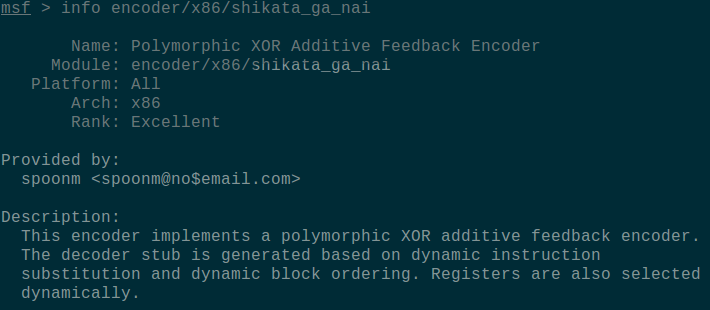
\includegraphics[width=\textwidth]{description.png}
\end{frame}

\begin{frame}{Shikata ga nai}
	\begin{itemize}
		\item 320 LoC
		\item Everyone patches it
		\item We want the original shellcode
	\end{itemize}
\end{frame}

\begin{frame}{Solutions}
	\begin{itemize}
		\item Run it as root on your machine
		\item Step-step-step-step-step-…
		\item Trace the execution in a virtual machine
		\item Use radare2\footnote{From git} ;)
	\end{itemize}
\end{frame}

\begin{frame}{ESIL}
	\begin{itemize}
		\item Evaluable String Intermediary Language
		\item Used for
			\begin{itemize}
				\item Emulation
				\item Decompilation\footnote{See radeco}
				\item Analysis
				\item Flamewars against other IL
			\end{itemize}
		\end{itemize}
\end{frame}

\begin{frame}{Where to stop?}
	We can emulate the shellcode, but where do we stop?
	\begin{itemize}
		\item Instructions aren't fixed
		\item Blocks are permutated
		\item Registers are dynamically selected
		\item{}
		\item So what can we do?
	\end{itemize}
\end{frame}

\begin{frame}{Reading the source code}
	It seems that the last instruction will always be \alert{loop}, and its counter in \alert{ecx}.
	\newline
	So we can emulate the shellcode, and dump the result at the last \alert{loop} instruction.
\end{frame}

\begin{frame}{r2pipe}
	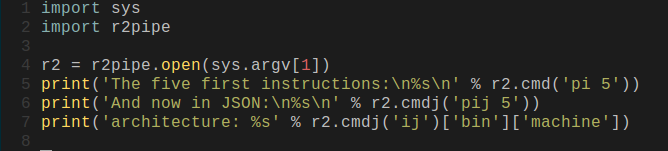
\includegraphics[width=\textwidth]{r2pipe.png}
\end{frame}

\begin{frame}{Initializing the ESIL VM}
	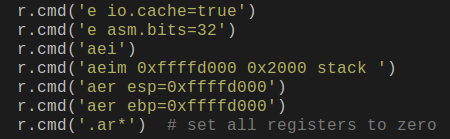
\includegraphics[width=\textwidth]{initmem.png}
\end{frame}

\begin{frame}{Plot twist}
	\only<1>{
		\begin{itemize}
			\item FPU is currently not supported in ESIL :D
			\item Only used to get EIP with \alert{FNSTENV}
			\item Polymorphic FPU instructions
		\end{itemize}
	}
	\only<2>{
		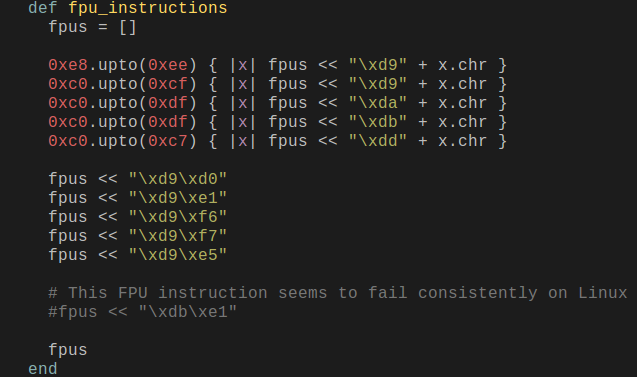
\includegraphics[width=\textwidth]{fpu.png}
	}
\end{frame}

\begin{frame}{Your turn!}
	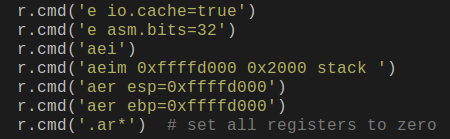
\includegraphics[width=\textwidth]{initmem.png}
\end{frame}

\section*{Conclusion}
\begin{frame}{Conclusion}
	\begin{center}
	\only<1>{
		\begin{itemize}
			\item ESIL is cool
			\item Still WIP
			\item More to come!
		\end{itemize}
	}
	\only<2>{
		\Large
		Radare2 is \alert{nice}.

		You should use it.
	}
	\end{center}
\end{frame}

\begin{frame}{Resources}
	\begin{itemize}
		\item \href{https://github.com/radare/radare2}{Github repo}
		\item \href{http://rada.re}{Official website}
		\item \href{http://radare.today}{The r2 blog}
		\item \href{http://maijin.github.io/radare2book/}{The r2 book}
		\item \href{https://twitter.com/radareorg}{Twitter}
	\end{itemize}
\end{frame}

\end{document}
